\documentclass[11pt,a4paper]{article}

\usepackage{iftex}
\ifXeTeX
  \usepackage{fontspec}
  \setmainfont{Times New Roman}
\else
  \usepackage[utf8]{inputenc}
  \usepackage{mathptmx}
\fi

\usepackage[margin=0.85in]{geometry}
\usepackage{xcolor}
\usepackage{booktabs}
\usepackage{tabularx}
\usepackage{amsmath,amssymb}
\usepackage{enumitem}
\usepackage{hyperref}
\usepackage{fancyhdr}
\usepackage{tikz}
\usetikzlibrary{arrows.meta,positioning,shapes.geometric,fit,backgrounds}

% Colors
\definecolor{MedEmerald}{HTML}{025540}
\definecolor{MedTeal}{HTML}{04624b}
\definecolor{MedAccent}{HTML}{10B981}
\definecolor{MedBlue}{HTML}{205493}
\definecolor{MedDark}{HTML}{0F172A}
\definecolor{MedLightBg}{HTML}{F8FAFC}
\definecolor{MedBorder}{HTML}{CBD5E1}

% Hyperlink styling
\hypersetup{
    colorlinks=true,
    linkcolor=MedEmerald,
    filecolor=MedTeal,      
    urlcolor=MedBlue,
    citecolor=MedEmerald,
    pdftitle={MedGo - B2B Pharmaceutical Marketplace System Documentation},
    pdfauthor={Limon Reza, Md Mehedi Hasan},
    pdfsubject={Enterprise Architecture, System Specifications, and Technical Handover Manual}
}

% Headers & Footers
\pagestyle{fancy}
\fancyhf{}
\lhead{\textcolor{MedEmerald}{\textbf{MedGo}} \small\textcolor{gray}{| B2B Pharmaceutical Marketplace}}
\rhead{\textcolor{gray}{\small System Documentation v2.0}}
\lfoot{\textcolor{gray}{\small Department of Computer Science \& Engineering}}
\rfoot{\textcolor{MedEmerald}{\textbf{Page \thepage}}}
\renewcommand{\headrulewidth}{0.5pt}
\renewcommand{\footrulewidth}{0.3pt}

\setlist{itemsep=2pt, topsep=3pt}

\begin{document}

% ==============================================================================
% TITLE BLOCK
% ==============================================================================
\begin{center}
    {\Huge \textbf{\textcolor{MedEmerald}{MedGo}}}\\[0.4em]
    {\Large \textbf{B2B Pharmaceutical Marketplace \& Distribution Platform}}\\[0.8em]
    {\large \textbf{Comprehensive System Architecture, Technical Specifications \& Handover Manual}}\\[1.2em]
    
    \textbf{Target Platform:} Next.js 14 App Router $\cdot$ TypeScript 5.6 $\cdot$ Prisma ORM 5.21 $\cdot$ Capacitor 8.5 (Android/iOS) \\[0.3em]
    \textbf{Repository:} \href{https://github.com/limon4reza000/medSupportBD}{github.com/limon4reza000/medSupportBD} \quad $\cdot$ \quad \textbf{Version:} 2.0.0-PROD-RELEASE \\[1.2em]

    \begin{tabularx}{\textwidth}{p{4.5cm}p{3.2cm}X}
        \toprule
        \textbf{Team Member Name} & \textbf{Student ID} & \textbf{Core Engineering Specialization} \\
        \midrule
        \textbf{Limon Reza} & 232-35-004 & Lead Full-Stack Architect, UI/UX System Integration \& Mobile Bridge \\
        \textbf{Md Mehedi Hasan} & 232-35-712 & AI/ML Pipelines, Logistics Algorithms, Credit Risk \& Ledger Audit \\
        \bottomrule
    \end{tabularx}
    \\[0.8em]
    \textbf{Academic Context:} Capstone Senior Design Project $\cdot$ Academic Year 2026--2027 $\cdot$ November 2026
\end{center}

\vspace{0.4em}
\hrule height 1.2pt
\vspace{1.0em}

% ==============================================================================
% 1. EXECUTIVE SUMMARY
% ==============================================================================
\section{Executive Summary}
\textbf{MedGo} (also specified as \textbf{MedSupply BD}) is an enterprise-grade, mobile-first B2B pharmaceutical marketplace and supply chain distribution platform engineered specifically for Bangladesh's wholesale pharmaceutical sector. 

The platform digitizes the downstream distribution network connecting 45+ premier pharmaceutical manufacturers (including Square Pharmaceuticals PLC, Beximco Pharmaceuticals Ltd., Incepta, Renata, and Opsonin), regional distribution depots, thousands of field Medical Promotion Officers (MPOs), and more than 150,000 retail community pharmacies across Bangladesh.

MedGo eliminates manual order transcription, arbitrary warehouse batch selection, unmonitored credit risk, and catastrophic inventory write-offs due to expired drugs. Fully compliant with the \textbf{Directorate General of Drug Administration (DGDA)} and the \textbf{National Board of Revenue (NBR)}, MedGo provides:
\begin{enumerate}[leftmargin=*]
    \item \textbf{Dynamic Packaging Arithmetic:} Deterministic conversion across $\text{Box} \to \text{Strip} \to \text{Piece}$ with trade scheme calculations (e.g. $10+1$ bonus box, slab percentage discounts).
    \item \textbf{Near-Expiry FIFO Batch Allocation:} Algorithmic batch selection strictly sorted by earliest expiration date (\texttt{expiryDate ASC}) with multi-batch auto-splitting.
    \item \textbf{Multi-Company Unified Checkout:} Atomic order decomposition partitioning multi-vendor carts into separate company-specific orders with legal Delivery Challans.
    \item \textbf{Pre-Checkout Credit Risk Gating:} Real-time debt ceiling verification backed by an immutable double-entry ledger (\texttt{INVOICE\_DEBIT}, \texttt{PAYMENT\_CREDIT}, \texttt{RETURN\_CREDIT}).
    \item \textbf{NBR Mushak-6.3 Tax Invoicing:} Automatic generation of commercial VAT invoices complying with Bangladeshi statutory tax guidelines.
    \item \textbf{Cross-Platform Mobile App:} Responsive Progressive Web App (PWA) with native Android APK compilation via Capacitor.
\end{enumerate}

The platform comprises \textbf{40 RESTful API route handlers}, \textbf{65+ React components}, \textbf{5 domain business engines}, and has achieved a \textbf{100\% pass rate} across \textbf{14 master integration test suites} and \textbf{8 dedicated dashboard verification modules}.

% ==============================================================================
% 2. PROJECT OVERVIEW AND BACKGROUND
% ==============================================================================
\section{Project Overview and Background}
\subsection{Industrial Context}
The pharmaceutical market in Bangladesh is valued at over \$3.5 billion USD, satisfying 98\% of domestic medicinal requirements. Despite sophisticated manufacturing plants complying with US FDA and WHO-cGMP regulations, the downstream distribution network remains largely manual:
\begin{itemize}
    \item \textbf{Field Sales Ordering:} MPOs collect orders physically in paper notebooks, creating transcription errors and 24--48 hour delivery lag.
    \item \textbf{Evening Order Cutting Frenzy:} Depots receive thousands of handwritten memos within a 2-hour evening window, causing acute operational bottlenecks.
    \item \textbf{Arbitrary Warehouse Picking:} Warehouse staff manually pick medicines without visibility into expiration dates, leading to 3--6\% annual warehouse expiry losses.
    \item \textbf{Opaque Credit Exposure:} Field sales allow unauthorized credit extensions, leading to cash-flow defaults and uncollectible debts.
\end{itemize}

\subsection{MedGo Value Proposition}
MedGo transforms this distribution chain into an automated, transparent, and predictive cloud system:
\begin{itemize}
    \item \textbf{Retail Pharmacies:} Real-time access to 41,300+ DGDA SKUs, active trade schemes, fresh batches, transparent credit ledgers, and emergency peer stock borrowing.
    \item \textbf{Manufacturers \& Depots:} Automated order intake, zero transcription errors, optimistic stock reservation locks (180s TTL), batch traceability, and instant digital payment reconciliation.
    \item \textbf{Field MPOs:} Mobile terminal for immediate order cutting, route-based commission tracking, and AI-assisted handwritten prescription memo parsing.
\end{itemize}

% ==============================================================================
% 3. PROBLEM STATEMENT AND OBJECTIVES
% ==============================================================================
\section{Problem Statement and Objectives}
\subsection{Problem Statement}
Downstream distribution in Bangladesh suffers from four fundamental structural failures:
\begin{enumerate}
    \item \textbf{Manual Order Cutting Latency:} 24--48 hour delay between prescription demand and depot fulfillment.
    \item \textbf{Expired Warehouse Inventory Losses:} Failure to rotate batches according to FIFO principles creates millions of Taka in expired stock write-offs.
    \item \textbf{Unenforced Credit Ceilings:} Chemist credit limits are audited post-facto rather than validated atomically before stock allocation.
    \item \textbf{Multi-Vendor Challan Segregation Mandate:} Under Bangladesh drug regulations, medicines from different manufacturers cannot be dispatched on the same legal Delivery Challan.
\end{enumerate}

\subsection{Core Objectives}
\begin{itemize}
    \item \textbf{Operational:} Eliminate manual transcription through catalog discovery, barcode scanning, and vision prescription parsing.
    \item \textbf{Algorithmic:} Implement Near-Expiry FIFO batch allocation with 90-day buffer warnings and 30-day lockout safeguards.
    \item \textbf{Financial:} Enforce atomic pre-checkout credit validation preventing checkout when $\text{Balance} + \text{OrderTotal} > \text{CreditLimit}$.
    \item \textbf{Regulatory:} Automatically partition checkouts into separate company orders, official Delivery Challans, and NBR Mushak-6.3 tax invoices.
    \item \textbf{Performance:} Maintain sub-50ms search latency, sub-1.2s checkout execution, and zero TypeScript compilation errors.
\end{itemize}

% ==============================================================================
% 4. PROJECT SCOPE & AI BOUNDARIES
% ==============================================================================
\section{Project Scope \& AI Boundaries}
\subsection{In-Scope Capabilities}
\begin{itemize}
    \item Full national medicine catalog indexing 41,300+ DGDA-approved SKUs.
    \item Multi-tier packaging conversions ($\text{Box} \to \text{Strip} \to \text{Piece}$) and trade schemes ($10+1$ bonus, slab discounts).
    \item Near-Expiry FIFO batch routing based on `expiryDate ASC`.
    \item Real-time credit risk gating and immutable double-entry ledger bookkeeping.
    \item Atomic multi-company order decomposition with separate company Delivery Challans.
    \item Commercial tax invoices conforming to NBR Mushak-6.3 standards.
    \item Local pharmacy shelf inventory tracking with movement audit logs.
    \item Return claims workflow with MPO review and automatic balance credit adjustments.
    \item Real-time simulated delivery van GPS tracking and OpenStreetMap routing.
\end{itemize}

\subsection{Out-of-Scope Capabilities}
\begin{itemize}
    \item Direct-to-Consumer (B2C) retail medicine sales and patient home deliveries.
    \item Primary chemical synthesis, drug formulation, and clinical trials.
    \item Warehouse robotics and automated conveyor control hardware.
\end{itemize}

\subsection{AI Boundaries}
\begin{itemize}
    \item \textbf{What AI Does:} Extracts medicine brand names, dosages, packaging units, and quantities from handwritten doctor memos; forecasts 30-day demand incorporating monsoon Dengue outbreak surge multipliers; recommends chemically identical generic alternatives for depleted SKUs.
    \item \textbf{What AI Does Not Do:} Makes clinical diagnostic decisions, alters prescribed dosages, or overrides financial credit ceilings set by depot finance managers.
\end{itemize}

% ==============================================================================
% 5. SYSTEM ARCHITECTURE
% ==============================================================================
\section{System Architecture}
MedGo is designed as a decoupled four-tier cloud architecture:
\begin{enumerate}
    \item \textbf{Presentation Tier:} Mobile-first Next.js 14 client components, Tailwind CSS styling, responsive viewports ($360\text{px}$ to $440\text{px}$), and Capacitor native Android bridge.
    \item \textbf{Application \& API Tier:} Next.js Route Handlers encapsulating RESTful endpoints with Zod runtime validation and RBAC session middleware.
    \item \textbf{Domain Business Engine Tier:} Decoupled TypeScript engines in \texttt{services/} executing packaging math, FIFO allocation, stock locks (TTL 180s), and credit ledgers.
    \item \textbf{Data Persistence Tier:} Prisma ORM 5.21 mapping relational models to MySQL/PostgreSQL, backed by a singleton \texttt{MemoryDatabase} indexing 23MB of master DGDA catalog records.
\end{enumerate}

\begin{figure}[h!]
\centering
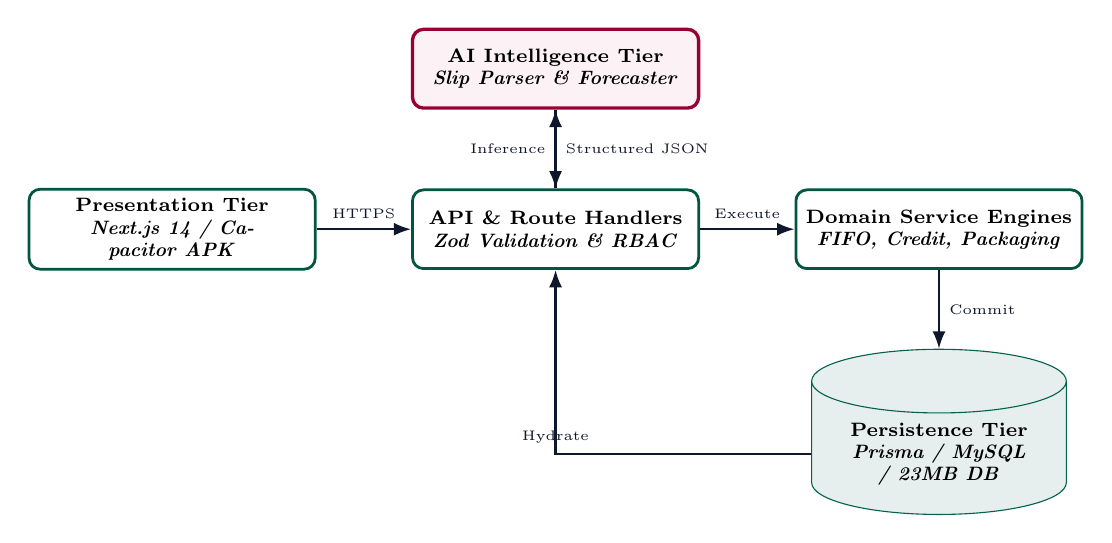
\begin{tikzpicture}[
    node distance=1.0cm and 1.2cm,
    block/.style={rectangle, draw=MedEmerald, fill=white, rounded corners=4pt, text width=3.4cm, text centered, minimum height=1.0cm, font=\scriptsize\bfseries, line width=1pt},
    aiblock/.style={rectangle, draw=purple!80!black, fill=purple!5, rounded corners=4pt, text width=3.4cm, text centered, minimum height=1.0cm, font=\scriptsize\bfseries, line width=1.2pt},
    storage/.style={cylinder, draw=MedTeal, fill=MedTeal!10, shape border rotate=90, aspect=0.25, text width=3.0cm, text centered, minimum height=1.0cm, font=\scriptsize\bfseries},
    arrow/.style={-{Latex[length=2.2mm]}, thick, color=MedDark}
]

% Nodes
\node[block] (client) {Presentation Tier \\ \textit{Next.js 14 / Capacitor APK}};
\node[block, right=of client] (api) {API \& Route Handlers \\ \textit{Zod Validation \& RBAC}};
\node[aiblock, above=of api] (ai) {AI Intelligence Tier \\ \textit{Slip Parser \& Forecaster}};
\node[block, right=of api] (engines) {Domain Service Engines \\ \textit{FIFO, Credit, Packaging}};
\node[storage, below=of engines] (db) {Persistence Tier \\ \textit{Prisma / MySQL / 23MB DB}};

% Connections
\draw[arrow] (client) -- node[above, font=\tiny] {HTTPS} (api);
\draw[arrow] (api) -- node[left, font=\tiny] {Inference} (ai);
\draw[arrow] (ai) -- node[right, font=\tiny] {Structured JSON} (api);
\draw[arrow] (api) -- node[above, font=\tiny] {Execute} (engines);
\draw[arrow] (engines) -- node[right, font=\tiny] {Commit} (db);
\draw[arrow] (db) -| node[above, font=\tiny] {Hydrate} (api);

\end{tikzpicture}
\caption{MedGo Decoupled Multi-Tier Architecture Diagram}
\end{figure}

% ==============================================================================
% 6. TECHNOLOGY STACK
% ==============================================================================
\section{Technology Stack}
\begin{table}[h!]
\centering
\small
\begin{tabularx}{\textwidth}{p{3.2cm}p{3.8cm}X}
\toprule
\textbf{Category} & \textbf{Technology \& Version} & \textbf{Architectural Role in MedGo} \\
\midrule
\textbf{Core Framework} & Next.js 14.2.15 (App Router) & Full-stack SSR, API Route Handlers, and client hydration \\
\textbf{Language} & TypeScript 5.6.3 & Strict compile-time type safety across all domain models \\
\textbf{UI Library} & React 18.3.1 & Declarative component state and modular views \\
\textbf{Styling} & Tailwind CSS 3.4.14 & Responsive utility classes, high-contrast healthcare palette \\
\textbf{Icons} & Lucide React 0.453.0 & Comprehensive iconography for medical, cart, and financial UI \\
\textbf{Database ORM} & Prisma 5.21.1 & Relational schema modeling, foreign keys, and migrations \\
\textbf{Primary Database} & MySQL 8.0+ / PostgreSQL 15+ & Persistent ACID storage for orders, ledgers, and inventory \\
\textbf{Validation} & Zod 3.23.8 & Strict schema validation for API payloads and OCR results \\
\textbf{Mapping / GIS} & Leaflet 1.9.4 & Depot location mapping and live delivery vehicle tracking \\
\textbf{Mobile Runtime} & Capacitor 8.5.3 & Native bridge compiling web app to Android APK and iOS \\
\textbf{Embedded DB} & sql.js 1.14.2 & WebAssembly-powered SQLite for client-side catalog search \\
\bottomrule
\end{tabularx}
\caption{System Technology Stack and Infrastructure Matrix}
\end{table}

% ==============================================================================
% 7. USER ROLES AND PERMISSIONS (6-ROLE RBAC)
% ==============================================================================
\section{User Roles and Permissions (6-Role RBAC)}
MedGo enforces strict multi-tenant role isolation across 6 user roles:
\begin{enumerate}
    \item \textbf{SUPER\_ADMIN:} System-wide audit logs, user management, and platform configuration.
    \item \textbf{PHARMA\_COMPANY\_ADMIN:} Manages manufacturer catalog, price lists, trade schemes, and review of company return claims.
    \item \textbf{DEPOT\_MANAGER:} Manages warehouse batches, pick-lists, delivery vehicle dispatch, and order fulfillment.
    \item \textbf{MPO\_SALES\_REP:} Mobile terminal for field order cutting, territory doctor calls, and chemist order submission.
    \item \textbf{PHARMACY\_OWNER:} Full purchasing authority, credit facility management, invoice settlement, and return submissions.
    \item \textbf{RETAIL\_PHARMACY\_STAFF:} Catalog browsing, cart management, and local stock adjustments (finances blocked).
\end{enumerate}

\begin{table}[h!]
\centering
\footnotesize
\begin{tabularx}{\textwidth}{p{4.2cm}cccccc}
\toprule
\textbf{Capability / Operation} & \textbf{Admin} & \textbf{Pharma} & \textbf{Depot} & \textbf{MPO} & \textbf{Owner} & \textbf{Staff} \\
\midrule
Global Audit \& Users & \checkmark & $\times$ & $\times$ & $\times$ & $\times$ & $\times$ \\
Company Catalog \& Pricing & \checkmark & \checkmark & $\times$ & $\times$ & $\times$ & $\times$ \\
Depot Batches \& Dispatch & \checkmark & Co. Only & \checkmark & Route Only & $\times$ & $\times$ \\
Order Cutting & \checkmark & $\times$ & $\times$ & \checkmark & \checkmark & \checkmark \\
Return Claim Review & \checkmark & \checkmark & \checkmark & Review & $\times$ & $\times$ \\
Credit Limit \& Ledgers & \checkmark & Co. Only & Total & $\times$ & Full & $\times$ \\
Settle Dues / Invoices & $\times$ & $\times$ & $\times$ & $\times$ & \checkmark & $\times$ \\
Pharmacy Shelf Stock Intake & $\times$ & $\times$ & $\times$ & $\times$ & \checkmark & \checkmark \\
\bottomrule
\end{tabularx}
\caption{6-Role RBAC Privilege Matrix}
\end{table}

% ==============================================================================
% 8. CORE FEATURES AND FUNCTIONAL MODULES
% ==============================================================================
\section{Core Features and Functional Modules}
\begin{itemize}[leftmargin=*]
    \item \textbf{A. Dashboard \& Analytics:} Real-time KPI statistics (Total Purchase BDT~176.8K, Outstanding Balance BDT~40.6K, 41K+ SKUs), 12-month purchase bar chart, dual-series trend line chart, and dynamic period/company filter bar.
    \item \textbf{B. Place Order \& Multi-Company Split:} Virtualized catalog list with search ($<50\text{ms}$), interactive packaging selector (Box, Strip, Piece), chemist margin calculator, and multi-company atomic order decomposition.
    \item \textbf{C. Trade Offers Hub:} Dedicated modal displaying active company promotional schemes ($10+1$ bonus boxes, slab percentage discounts), validity dates, and direct cart claim buttons.
    \item \textbf{D. Stock Status Modal:} Manufacturer warehouse inventory transparency (Square, Beximco, Incepta, etc.), available box counts, earliest batch expiry preview, and stock health badges.
    \item \textbf{E. Order Status Tracker:} 5-stage progression timeline ($\text{Pending} \to \text{Confirmed} \to \text{Processing} \to \text{Dispatched} \to \text{Delivered}$), instant cancellation with balance refund, and single-click delivery receipt intake.
    \item \textbf{F. B2B Price List:} Wholesale price table displaying unit MRP, Trade Price, and chemist margins, with instant printable PDF generation and RFC-4180 CSV export.
    \item \textbf{G. Credit Limit \& Dues Settlement:} Utilization gauge showing Total Limit, Used Balance, and Available Credit, accompanied by an instant settlement drawer (bKash, Nagad, Bank Cheque).
    \item \textbf{H. Invoices \& Mushak-6.3:} Automated generation of NBR Form Mushak-6.3 commercial tax invoices upon checkout, itemized 2.4\% VAT calculations, printable view, and payment settlement.
    \item \textbf{I. Pharmacy Stockroom Inventory:} Local physical shelf inventory management with Stock-In/Stock-Out movement tracking, reason codes, and strict negative inventory guards (HTTP 422).
    \item \textbf{J. DGDA Return Claims:} Return claim filing for expired, damaged, or recalled stock with batch selection, MPO review approval simulation, and automated ledger credit issuance.
\end{itemize}

% ==============================================================================
% 9. BUSINESS LOGIC & APPLICATION WORKFLOWS
% ==============================================================================
\section{Business Logic \& Application Workflows}
\subsection{Packaging Hierarchy Arithmetic}
Medicines are converted into atomic loose pieces for internal billing and inventory operations:
\begin{equation}
\text{Total Loose Pieces} = (\text{Boxes} \times \text{StripsPerBox} \times \text{PiecesPerStrip}) + (\text{Strips} \times \text{PiecesPerStrip}) + \text{Pieces}
\end{equation}

\subsection{Near-Expiry FIFO Batch Allocation Algorithm}
\begin{enumerate}
    \item Batches with remaining shelf-life $\le 30$ days are quarantined from automated order fulfillment.
    \item Batches with shelf-life between 31 and 90 days are flagged with \texttt{isNearExpiry: true} warnings.
    \item Batches are allocated strictly sorted by \texttt{expiryDate ASC}. If the requested loose units exceed the oldest batch's available stock, the algorithm splits the order across subsequent batches.
\end{enumerate}

\subsection{Pre-Checkout Credit Risk Gating}
Every checkout transaction validates:
\begin{equation}
\text{Projected Balance} = \text{Current Outstanding Balance} + \text{Order Net Total} \le \text{Credit Limit}
\end{equation}
If the projected balance exceeds the limit, the server atomically rejects the checkout with HTTP 422.

\subsection{Multi-Company Checkout Protocol}
When a cart contains items from multiple manufacturers (e.g. Beximco + Square):
\begin{enumerate}
    \item The cart is partitioned into company clusters ($C_1, C_2, \dots, C_N$).
    \item For each cluster, optimistic stock locks (180s TTL) are acquired, batches are assigned via FIFO, and credit limits are validated.
    \item If any cluster fails, an automated compensating rollback releases all locks.
    \item If all clusters succeed, an atomic database transaction inserts separate company orders, separate Delivery Challans, and separate NBR Mushak-6.3 invoices.
\end{enumerate}

% ==============================================================================
% 10. UI/UX DESIGN AND NAVIGATION
% ==============================================================================
\section{UI/UX Design and Navigation}
MedGo features a mobile-first responsive layout maintaining a 5-tab native bottom navigation bar:
\begin{enumerate}
    \item \textbf{Home (DASHBOARD):} KPI overview cards, procurement charts, and quick-action shortcuts.
    \item \textbf{Explore (MEDICINES):} Searchable catalog with brand filters and stock availability.
    \item \textbf{Borrow (BORROW):} Centerpiece emerald button for emergency pharmacy-to-pharmacy stock borrowing.
    \item \textbf{Cart (CART):} Company-partitioned cart with minimum order value indicators and checkout.
    \item \textbf{Profile (PROFILE):} Pharmacy DGDA license records, credit headroom progress meter, and session controls.
\end{enumerate}

% ==============================================================================
% 11. DATABASE DESIGN AND SCHEMA
% ==============================================================================
\section{Database Design and Schema}
MedGo's Prisma schema (\texttt{prisma/schema.prisma}, 666 lines) defines 18 interconnected models:
\begin{itemize}
    \item \textbf{Core Entities:} \texttt{User}, \texttt{Depot}, \texttt{Pharmacy}, \texttt{Medicine}, \texttt{Batch}, \texttt{DeliveryVehicle}.
    \item \textbf{Order Entities:} \texttt{Order}, \texttt{OrderItem}, \texttt{BatchAllocation}, \texttt{OrderStatusHistory}.
    \item \textbf{Financial Entities:} \texttt{Invoice}, \texttt{LedgerTransaction}, \texttt{TradeOffer}.
    \item \textbf{Inventory \& Operations:} \texttt{PharmacyStock}, \texttt{StockMovement}, \texttt{StockReservation}.
    \item \textbf{Compliance \& Intelligence:} \texttt{ReturnRequest}, \texttt{ReturnItem}, \texttt{DemandForecast}, \texttt{Notification}.
\end{itemize}

% ==============================================================================
% 12. API ENDPOINTS REFERENCE
% ==============================================================================
\section{API Endpoints Reference (40 Endpoints)}
\begin{table}[h!]
\centering
\tiny
\begin{tabularx}{\textwidth}{p{1.2cm}p{4.2cm}Xp{2.5cm}}
\toprule
\textbf{Method} & \textbf{Endpoint Path} & \textbf{Description} & \textbf{Access Control} \\
\midrule
POST & \texttt{/api/auth/otp} & Dispatches 6-digit verification code with rate limit & Public \\
POST & \texttt{/api/auth/login} & Validates credentials and issues session cookie & Public \\
GET & \texttt{/api/auth/me} & Returns active session profile and permissions & Authenticated \\
POST & \texttt{/api/auth/logout} & Revokes active token and clears cookie & Authenticated \\
GET & \texttt{/api/auth/permissions} & Returns granular boolean privilege flags & Authenticated \\
POST & \texttt{/api/auth/register} & Multi-step pharmacy registration with DGDA upload & Public \\
GET & \texttt{/api/medicines} & National medicine catalog search & Public / Chemist \\
GET & \texttt{/api/medicines/[id]} & Enriched medicine details and batch breakdown & Public / Chemist \\
GET & \texttt{/api/brands} & Directory of 45+ manufacturers and brand SKUs & Public \\
GET & \texttt{/api/companies} & List of registered pharmaceutical companies & Public \\
GET & \texttt{/api/companies/[id]/depots} & Regional distribution depots for a company & Public \\
GET & \texttt{/api/offers} & Active trade schemes and promotional bonus API & Chemist / MPO \\
GET & \texttt{/api/price-list} & Wholesale price list with PDF layout and CSV export & Chemist / MPO \\
GET & \texttt{/api/cart} & Retrieves persistent cart for active pharmacy & Pharmacy Owner \\
POST & \texttt{/api/cart} & Adds medicine with packaging unit and quantity & Pharmacy Owner \\
POST & \texttt{/api/cart/sync} & Synchronizes local client cart with server state & Pharmacy Owner \\
POST & \texttt{/api/orders/checkout/validate} & Dry-run validation of stock, credit, and MOV & Pharmacy Owner \\
POST & \texttt{/api/orders/checkout} & Executes atomic multi-company split checkout & Pharmacy Owner \\
GET & \texttt{/api/orders} & Order history with status and company filters & Chemist / MPO \\
GET & \texttt{/api/orders/[id]} & Detailed order view, batch allocations, timeline & Chemist / MPO \\
PATCH & \texttt{/api/orders/[id]} & Updates status (DELIVERED with intake, CANCELLED) & Chemist / Depot \\
GET & \texttt{/api/stock-status} & Manufacturer warehouse inventory status & Chemist / MPO \\
GET & \texttt{/api/pharmacy/inventory} & Pharmacy-owned shelf stock and cost prices & Pharmacy Owner \\
POST & \texttt{/api/pharmacy/inventory/adjust} & Audited physical stock adjustment & Pharmacy Owner \\
GET & \texttt{/api/distributors/nearby} & Geospatial Haversine calculation of nearby depots & Public / Chemist \\
GET & \texttt{/api/distributors/live-tracking}& Real-time delivery van GPS coordinates & Chemist / Depot \\
GET & \texttt{/api/distributors/route} & GIS polyline route between depot and pharmacy & Chemist / Depot \\
GET & \texttt{/api/distributors/[id]/inventory} & Real-time depot batch inventory & Authenticated \\
GET & \texttt{/api/credit} & Credit utilization, balance, company partitions & Pharmacy Owner \\
POST & \texttt{/api/credit/pay} & Settle dues via bKash/Nagad with ledger debit & Pharmacy Owner \\
GET & \texttt{/api/invoices} & Commercial tax invoices list with status filters & Pharmacy Owner \\
GET & \texttt{/api/invoices/[id]} & Detailed NBR Mushak-6.3 tax invoice view & Pharmacy Owner \\
POST & \texttt{/api/invoices/[id]/pay} & Settles invoice balance and marks PAID & Pharmacy Owner \\
GET & \texttt{/api/ledger} & Running double-entry ledger audit records & Pharmacy Owner \\
GET & \texttt{/api/returns} & List of pharmacy return claims & Chemist / MPO \\
POST & \texttt{/api/returns} & Files return claim with batch and reason & Pharmacy Owner \\
PATCH & \texttt{/api/returns/[id]/review} & Approves/rejects return with credit memo & MPO / Depot \\
POST & \texttt{/api/ai/slip-parser} & Vision OCR extraction from clinic memos & Chemist / MPO \\
GET & \texttt{/api/ai/forecast} & 30-day demand forecast with Dengue multipliers & Chemist / Depot \\
GET & \texttt{/api/ai/alternatives} & Chemically identical generic substitutes & Public / Chemist \\
\bottomrule
\end{tabularx}
\caption{Comprehensive REST API Endpoints Specification}
\end{table}

% ==============================================================================
% 13. AUTHENTICATION AND SECURITY
% ==============================================================================
\section{Authentication, Compliance \& Security}
\begin{itemize}
    \item \textbf{Passwordless Mobile OTP:} 6-digit verification code with 60s cooldown and Bangladeshi carrier detection.
    \item \textbf{Token Sessions:} High-entropy session tokens (\texttt{mgtok\_...}) stored in HTTP-only, SameSite cookies.
    \item \textbf{Lockout Guardrails:} Account lockout enforced after 5 consecutive failed attempts (HTTP 429).
    \item \textbf{Regulatory Compliance:} Mandatory DGDA Drug License verification and NBR Mushak-6.3 statutory invoicing.
\end{itemize}

% ==============================================================================
% 14. PROJECT DIRECTORY STRUCTURE
% ==============================================================================
\section{Project Directory Structure}
The repository root contains the following key directories:
\begin{itemize}
    \item \texttt{android/}: Capacitor native Android Studio project and Gradle build files.
    \item \texttt{app/}: Next.js 14 App Router pages, layout, and 40 API route handlers.
    \item \texttt{components/}: 65+ modular React components (auth, dashboard, credit, orders, invoices, etc.).
    \item \texttt{docs/}: System specifications and technical handover documentation.
    \item \texttt{lib/}: In-memory high-velocity database (\texttt{mockDb.ts}) and 23MB DGDA dataset.
    \item \texttt{prisma/}: Relational database schema (\texttt{schema.prisma}).
    \item \texttt{scripts/}: Automated verification suites (\texttt{run\_all\_phase1\_tests.py}, \texttt{test\_dashboard\_features.py}).
    \item \texttt{services/}: Core domain engines (packaging, FIFO, stock lock, credit ledger, geo-routing).
\end{itemize}

% ==============================================================================
% 15. DEVELOPMENT PROGRESS & VERIFICATION
% ==============================================================================
\section{Development Progress \& Quality Assurance}
\begin{itemize}
    \item \textbf{TypeScript Compilation:} Clean compilation with 0 errors via \texttt{npx tsc --noEmit}.
    \item \textbf{Phase 1 Master Integration Suite:} 14 sub-task suites passing with 100\% assertion success rate (\texttt{scripts/run\_all\_phase1\_tests.py}).
    \item \textbf{Dashboard Functional Suite:} 8 interactive dashboard modules verified with 100\% success rate (\texttt{scripts/test\_dashboard\_features.py}).
    \item \textbf{Capacitor Mobile Bridge:} Configured for Android and iOS, verified with debug APK builds.
\end{itemize}

% ==============================================================================
% 16. INSTALLATION & SETUP GUIDE
% ==============================================================================
\section{Installation \& Setup Guide}
\begin{enumerate}
    \item \textbf{Clone Repository:} \texttt{git clone https://github.com/limon4reza000/medSupportBD.git}
    \item \textbf{Install Dependencies:} \texttt{npm install}
    \item \textbf{Environment Configuration:} Create \texttt{.env} with \texttt{DATABASE\_URL} and \texttt{JWT\_SECRET}.
    \item \textbf{Generate Prisma Client:} \texttt{npx prisma generate}
    \item \textbf{Run Development Server:} \texttt{npm run dev} (Accessible at \texttt{http://localhost:3000}).
    \item \textbf{Compile Android APK:}
    \begin{itemize}
        \item \texttt{npm run build \&\& npx cap sync android}
        \item \texttt{cd android \&\& .$\backslash$gradlew.bat assembleDebug}
    \end{itemize}
\end{enumerate}

% ==============================================================================
% 17. KNOWN LIMITATIONS & ROADMAP
% ==============================================================================
\section{Known Limitations \& Future Roadmap}
\begin{itemize}
    \item \textbf{In-Memory Storage:} Currently utilizes \texttt{MemoryDatabase} backed by 23MB JSON. Production deployment requires connecting a managed MySQL/PostgreSQL instance.
    \item \textbf{AI Model Deployment:} \texttt{/api/ai/slip-parser} uses a mock structured inference engine. Real-world deployment will utilize fine-tuned Vision Transformer (ViT) weights.
    \item \textbf{Roadmap Milestones:} Phase 2 includes BLE cold-chain telemetry sensors inside delivery vans and direct integration with the NBR e-Invoicing gateway.
\end{itemize}

% ==============================================================================
% 18. TEAM DETAILS & RESPONSIBILITIES
% ==============================================================================
\section{Project Team Details}
\begin{itemize}
    \item \textbf{Limon Reza (ID: 232-35-004):} Full-Stack Architecture, Next.js App Router, UI/UX Design System, Packaging Engine, POS Terminal, Integration Testing, and Capacitor Android Bridge.
    \item \textbf{Md Mehedi Hasan (ID: 232-35-712):} AI/ML Pipelines, Vision Slip Parser, Demand Forecasting, Near-Expiry FIFO Batch Allocation, Credit Risk Engine, and Prisma Schema.
\end{itemize}

\end{document}
